\title{linear equations in two variables}
%\usepackage{graphicx} % Required for inserting images

\documentclass[12pt]{article}
\usepackage{amsmath}
\newcommand{\myvec}[1]{\ensuremath{\begin{pmatrix}#1\end{pmatrix}}}
\newcommand{\mydet}[1]{\ensuremath{\begin{vmatrix}#1\end{vmatrix}}}
\newcommand{\solution}{\noindent \textbf{Solution: }}
\providecommand{\brak}[1]{\ensuremath{\left(#1\right)}}\providecommand{\norm}[1]{\left\lVert#1\right\rVert}
\let\vec\mathbf
\usepackage{float}
\usepackage{graphicx}

\title{Coordinate Geometry}
\author{VADDI SRIKARAN (vaddisrikaran@sriprakashschools.com)}
\begin{document}
\maketitle
\section*{10$^{th}$ Maths - Chapter 7}
This is Problem-4 from Exercise 7.1
\begin{enumerate}
\item Check whether (5, – 2), (6, 4) and (7, – 2) are the vertices of an isosceles triangle. \\
\solution:\\
Given,
\begin{align}
\vec{A}&=\myvec{5\\-2}\\
\vec{B}&=\myvec{6\\4}\\
\vec{C}&=\myvec{7\\-2}\\
\vec{AB}&=\myvec{1\\6}\\
\norm{AB}&=\sqrt{(1)^2+(6)^2}\\
&=\sqrt{37}\\
\norm{BC}&=\sqrt{(1)^2+(-6)^2}\\
&=\sqrt{37}\\
\norm{CA}&=\sqrt{(2)^2+0}\\
&=\sqrt{4}\\
\end{align}
since,$|AB|$=$|BC|$=$\sqrt{37}$,they are isosceles triangle
\end{enumerate}
\begin{figure}[H]
			\centering
			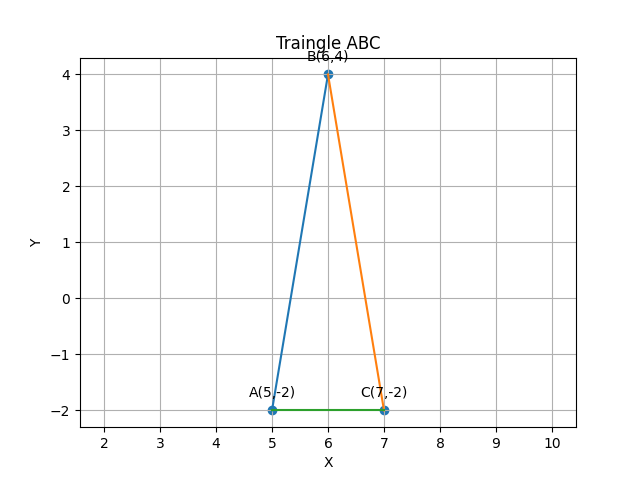
\includegraphics[width=\columnwidth]{figs/Figure_1.png}
			\caption{Triangle ABC}
			\label{fig:10}
   \end{figure}
\end{document}
\end{document}
